%=====================================================================
\section{Learning the model error: residual Koopman models (RQ1)}\label{sec:koopman}
%=====================================================================
This section answers the prediction half of RQ1: which model best predicts how the failed drone will move? We compare three predictors trained and tested on exactly the same data (experiment E6).

\subsection{Hypotheses}
Before running the experiment we wrote down what we expected (from the proposal):
\begin{description}[leftmargin=1.2em]
  \item[H1.] A Koopman model of the full dynamics, learned from failed-drone data, has eigenvalues outside the unit circle and loses to a trivial ``nothing changes'' predictor at long horizons. (Our proposal found this for a healthy drone.)
  \item[H2.] The residual model has a lower multi-step prediction error than both the physics model and the full Koopman model.
  \item[H4.] The residual model reaches a given error with less data than the full Koopman model. (H3 concerns MPC and is tested in Section~\ref{sec:mpc}.)
\end{description}

\subsection{Data}
\paragraph{Why a separate truth plant.} The data come from truth plant A (Section~\ref{sec:truth}), not from the nominal model. Otherwise the physics model would already be perfect and there would be nothing to learn.

\paragraph{How episodes are generated.} Each episode lasts 4\,s with rotor 4 failed:
\begin{enumerate}
  \item The drone starts near the relaxed hover, with random deviations drawn uniformly: body rates $\pm2$\,rad/s, tilt $\pm0.15$ in $n_x$ and $n_y$, height and vertical speed $\pm0.5$.
  \item It is flown by the failure LQR designed on the \emph{nominal} parameters. A learned model needs to see the drone respond to many different inputs, so we add a random \emph{excitation}: every 50\,ms a new random offset, uniform in $\pm0.35$\,N, is added to each of the three thrust commands (then clipped to the limits).
  \item The simulator runs at 1\,ms; the controller and the recorded data run at $\Ts = 5$\,ms.
  \item At every sample we record the measured state as a deviation from the relaxed hover, $\vect x = (p,q,r,n_x,n_y,z,v_z) - \bar{\vect s}$; the command deviation $\vect u = (f_1,f_2,f_3) - \bar{\vect f}$; and $\hat{\vect f}$, the nominal first-order filter of the commands. The true motor thrust is not used, because a real flight computer does not measure it.
  \item Episodes in which the tilt deviation exceeds 0.6 (the drone has left the region of interest) are discarded.
\end{enumerate}
Training uses 40 episodes (32,000 samples, seed 11). Testing uses 10 new episodes from plant A (seed 12) and 10 from the held-out plant B (seed 13). A second training set of 40 episodes, each from a randomly drawn plant (seed 21), tests whether varied training data helps.

\subsection{The three predictors}
\paragraph{1. Analytical (physics only).} The 10-state linear model of Section~\ref{sec:linmodels} (7 states and 3 motor states, nominal parameters), discretized exactly with a zero-order hold at 5\,ms:
\begin{equation}
  \vect s_{k+1} = A_d\vect s_k + B_d\vect u_k, \qquad \vect s = (\vect x, \hat{\vect f}) \in\mathbb R^{10}.
\end{equation}
It uses no data at all.

\paragraph{2. Full-state EDMDc.} Everything is learned from data~\cite{williams2015edmd,korda2018linear}. We take the 9-number vector $\vect\xi = (p,q,r,n_x,n_y,v_z,\hat f_1,\hat f_2,\hat f_3)$; height $z$ is left out because it is just the integral of $v_z$. Each entry is \emph{standardized} (the training mean subtracted and the result divided by the training standard deviation), giving $\tilde{\vect\xi}$. The dictionary is
\begin{equation}
  \psi(\vect\xi) = \big(\;1,\;\; \tilde\xi_1,\dots,\tilde\xi_9,\;\; \tilde\xi_1^2,\, \tilde\xi_1\tilde\xi_2,\,\dots,\,\tilde\xi_9^2\;\big),
\end{equation}
that is, a constant, the 9 standardized values and all 45 products of two of them: $1 + 9 + 45 = 55$ functions. We then fit the lifted linear model
\begin{equation}
  \psi(\vect\xi_{k+1}) \approx A\,\psi(\vect\xi_k) + B\,\vect u_k
\end{equation}
by ridge regression over all training pairs (regularization $\lambda = 10^{-6}$). To predict, we lift the starting state once, iterate $\vect\zeta\leftarrow A\vect\zeta + B\vect u$ (we write $\vect\zeta$ for the lifted state here, to avoid confusion with the height $z$), read $\vect\xi$ back from the 9 linear coordinates of $\vect\zeta$, and integrate $v_z$ with the trapezoid rule to get the height $z$.

\paragraph{3. Residual EDMDc (proposed).} Keep the physics model and learn only its one-step error. For every training pair we compute what the physics model would have predicted and the difference to what really happened:
\begin{equation}
  \vect e_{k+1} = \vect x_{k+1} - \big[A_d\vect s_k + B_d\vect u_k\big]_{1:7}.
\end{equation}
We regress $\vect e_{k+1}$ on the same kind of quadratic dictionary, now built from $(\vect\xi_k, \vect u_k)$ (the same 9 values plus the 3 commands, standardized; $1 + 12 + 78 = 91$ functions), with ridge regularization $\lambda = 10^{-3}$, giving a matrix $W$. The prediction is
\begin{equation}
  \vect x_{k+1} = \big[A_d\vect s_k + B_d\vect u_k\big]_{1:7} + \operatorname{clip}\big(W^\top\psi(\vect\xi_k,\vect u_k),\; \pm\vect d_{\max}\big),
\end{equation}
where $\vect d_{\max}$ is the 99.5th percentile of the absolute training residuals, per state. The clipping, borrowed from Todde et al.~\cite{todde2026residual}, prevents the learned part from producing a correction larger than anything seen in training, for example when the drone is far from the training data.

\paragraph{Why we call it a residual Koopman model.} Strictly, this model uses the EDMD dictionary and least squares to learn a \emph{one-step} correction; unlike the full-state EDMDc model it does not propagate a lifted linear state, and the input enters it nonlinearly (through products such as $\xi_i u_j$). It is closer to a polynomial regression of the error than to a linear Koopman predictor, and we keep the name only because it follows the same construction as the residual models in the literature~\cite{todde2026residual,narayanan2026rkmpc}. What keeps the MPC problem convex is not linearity of this model but the way it is used: it is evaluated outside the optimization (Section~\ref{sec:mpc}).

\begin{plain}
The physics model provides most of the prediction: it already knows that the drone spins, how fast, and how it responds to each rotor. The learned part only has to describe a small correction, such as ``the drone sinks a little faster than the physics says when it spins fast'', and that correction is much easier to learn than the whole motion.
\end{plain}

\begin{codebox}{fitting the residual}
\begin{lstlisting}
for X, fe, U in zip(data.x, data.fe, data.u):          # every training episode
    for k in range(len(U)):
        x1n, _ = nom.step(X[k], fe[k], U[k])            # physics prediction
        E.append(X[k + 1] - x1n)                        # what it got wrong
        F.append(np.concatenate((X[k, XI_IDX], fe[k], U[k])))
dic = Dictionary(F.mean(0), F.std(0) + 1e-9)           # standardize, quadratic features
W = ridge(dic(F), E, lam)                               # (Phi'Phi + lam I)^-1 Phi'E
d_max = np.percentile(np.abs(E), 99.5, axis=0)          # clipping level
\end{lstlisting}
\end{codebox}

\paragraph{4. No-change baseline.} The prediction is simply the starting state, held forever. Any model worse than this is useless at that horizon.

\subsection{How prediction error is measured}
From each test episode (800 samples) we start a prediction every 40 samples (0.2\,s), as long as the longest horizon (600 samples) still fits: 5 starts per episode, all in the first 0.8\,s, so 50 starts per test set. Each predictor is given the true starting state and the recorded inputs, and it predicts \emph{open loop}, that is, without seeing any later measurement. We compare the prediction with the true trajectory at horizons from 5\,ms to 3\,s. Each state's error is divided by that state's standard deviation in the training data (so rad/s and metres can be combined), squared, averaged over all start times and all 7 states, and square-rooted:
\begin{equation}
  \text{NRMSE}(h) = \sqrt{\frac{1}{7N_{\text{starts}}}\sum_{\text{starts}}\sum_{i=1}^{7}\left(\frac{\hat x_i(h) - x_i(h)}{\operatorname{std}_i}\right)^2 }.
\end{equation}
(To keep a diverging model from producing overflow, each squared error is capped at $10^{12}$ before averaging.) A value of 1 means the error is as large as the typical variation of the states; the no-change baseline sits at about 2.4.

\subsection{Results}
\begin{table}[h]
\centering\small
\caption{Normalized multi-step prediction error (lower is better), models trained on family A.}\label{tab:pred}
\begin{tabular}{lccccccc}
\toprule
& \multicolumn{4}{c}{Test family A} & \multicolumn{3}{c}{Test family B (held out)} \\
\cmidrule(lr){2-5}\cmidrule(lr){6-8}
Predictor & 20\,ms & 0.1\,s & 1\,s & 2\,s & 0.1\,s & 1\,s & 2\,s \\
\midrule
Analytical & 0.65 & 3.17 & 7.09 & 7.93 & 4.31 & 7.94 & 6.95 \\
Full-state EDMDc & \textbf{0.04} & 0.17 & 0.91 & 3.45 & 6.09 & 26.2 & 131 \\
Residual EDMDc & 0.10 & \textbf{0.15} & \textbf{0.64} & 2.71 & 5.98 & 19.9 & 24.0 \\
No change & 0.81 & 2.42 & 2.38 & 2.51 & 2.51 & 2.44 & 2.41 \\
\bottomrule
\end{tabular}
\end{table}

\begin{figure}[h]
\centering
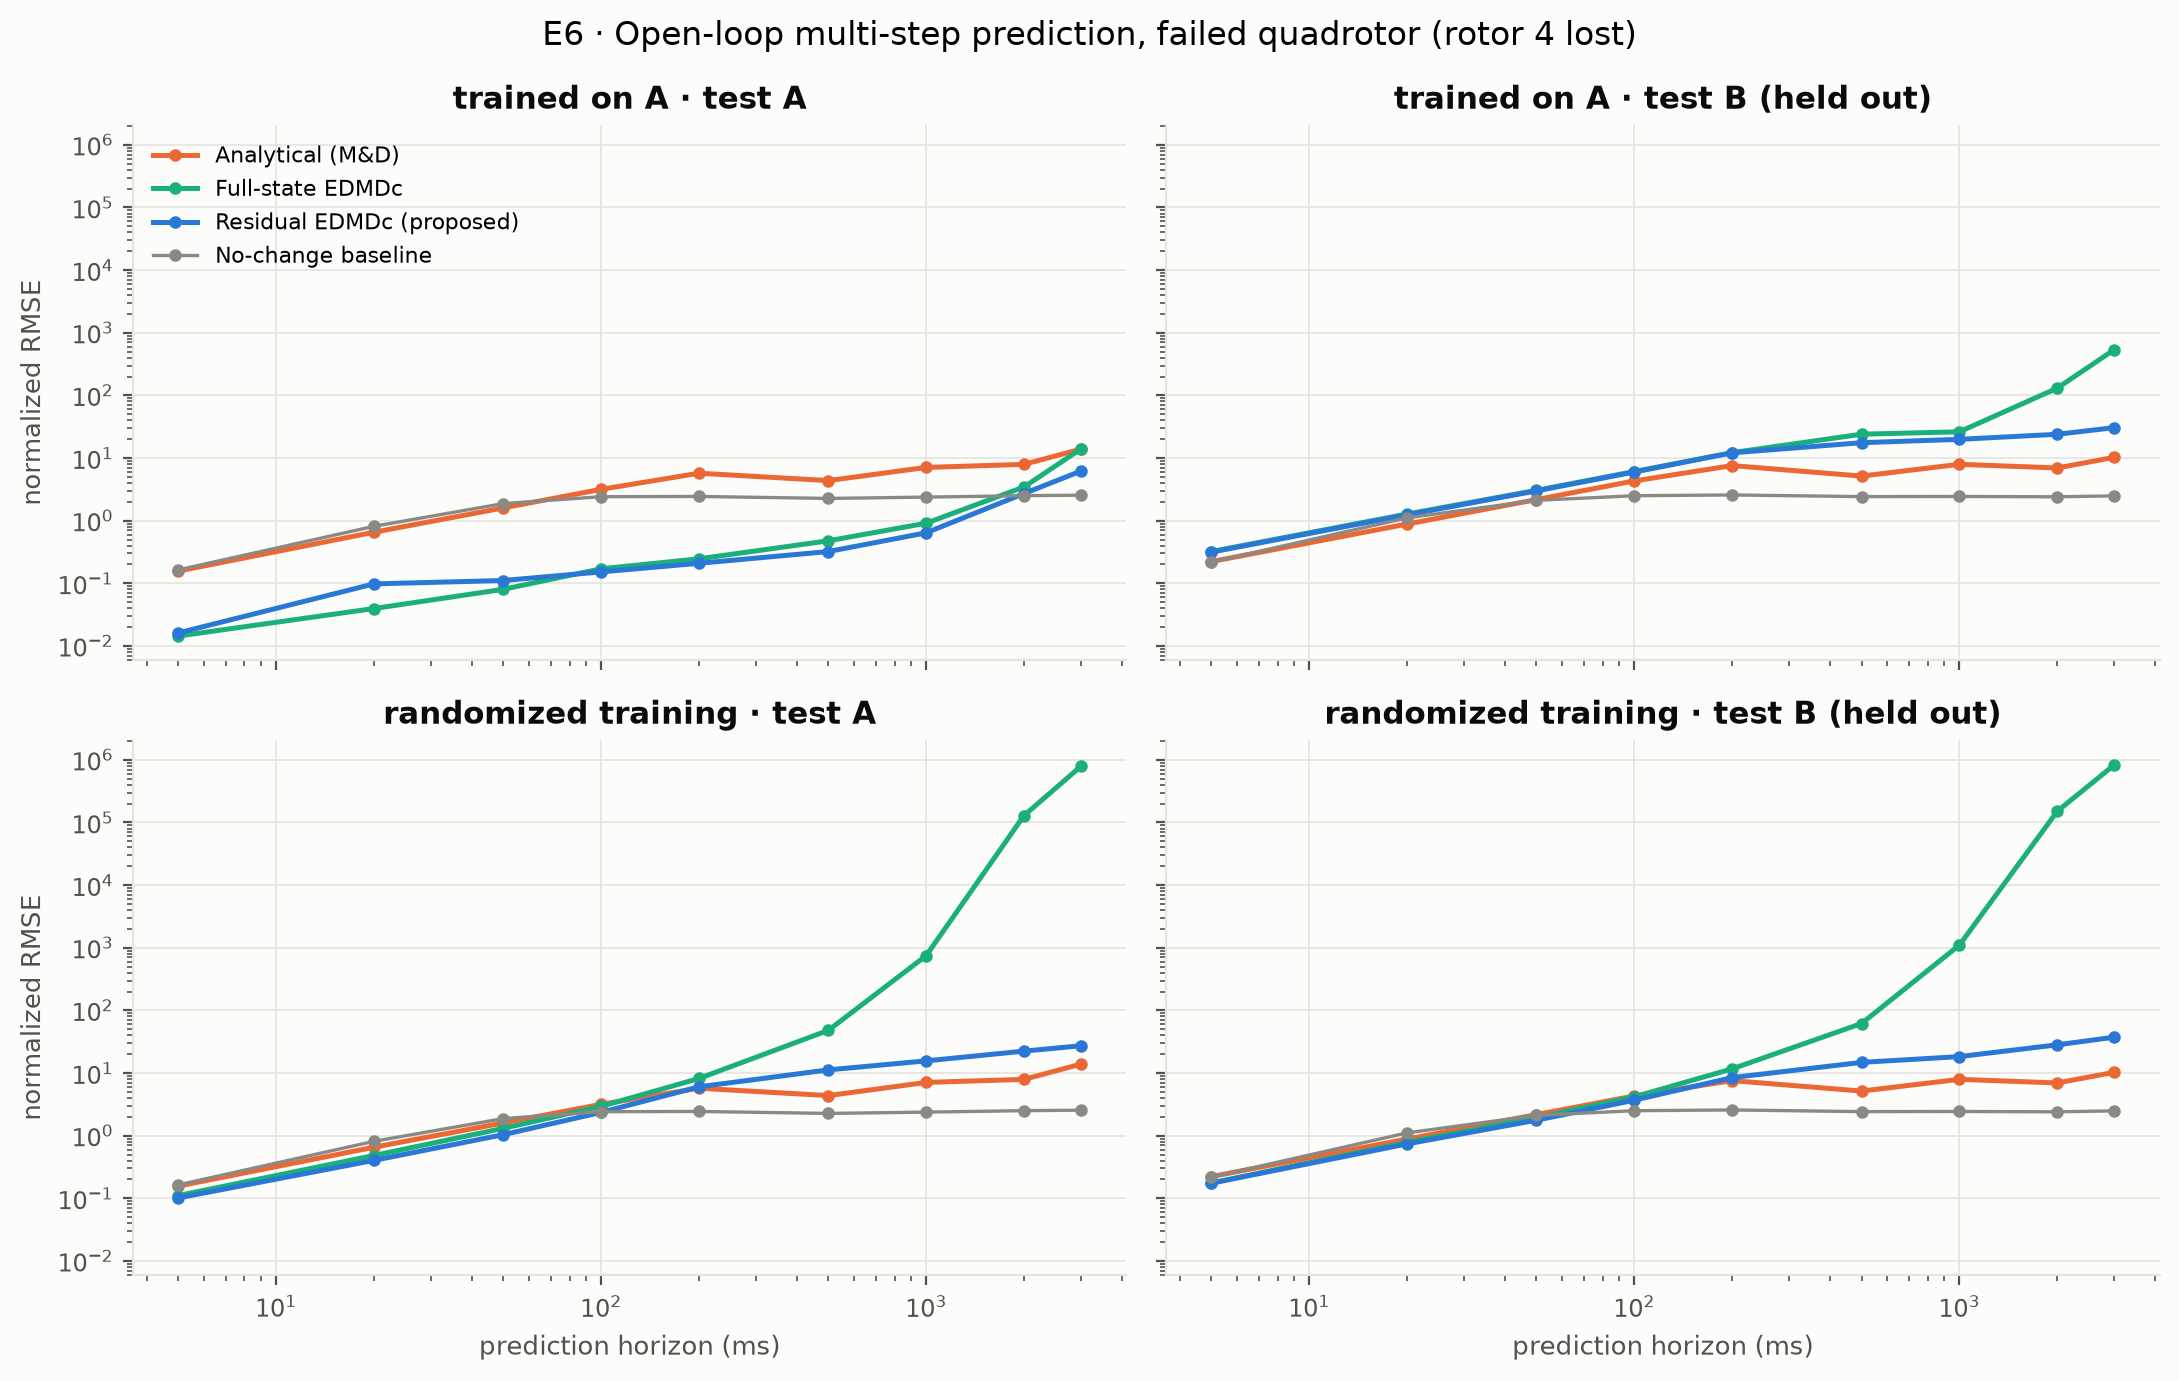
\includegraphics[width=0.95\linewidth]{figures/e6_multistep_error.png}
\caption{Multi-step prediction error against horizon (both axes logarithmic). Top: trained on family A. Bottom: trained on randomized plants. Left: tested on family A; right: tested on the held-out family B.}\label{fig:pred}
\end{figure}

\paragraph{H2 (residual is best): supported on the training plant.} On new episodes from plant A, the residual model is the most accurate of the three models at every horizon from 100\,ms on, and the most accurate predictor overall from 100\,ms to 1\,s (Table~\ref{tab:pred}, Figure~\ref{fig:pred} top left). At 1\,s its error is 0.64, against 0.91 for full-state EDMDc and 7.09 for the physics model. At short horizons (5 to 50\,ms) the full-state model is better, by a factor of 2.5 at 20\,ms (0.04 against 0.10). The physics model is worse than the no-change baseline from about 100\,ms on: its undamped modes and the unmodelled thrust loss make it drift away. At 2\,s even the residual model is behind the no-change baseline, so long open-loop horizons need feedback, which is what MPC provides by re-planning every 5\,ms.

\paragraph{H1 (full model is unstable): supported.} The learned $55\times55$ matrix $A$ of the full-state model has 4 eigenvalues outside the unit circle (spectral radius 1.0070, Figure~\ref{fig:eigs}). The true open-loop model has undamped modes that lie exactly on the unit circle in discrete time, so this is a small outward push of modes that are only marginally stable in reality, not a qualitatively different defect. Over many steps, however, it makes errors grow, and the model falls behind the no-change baseline by 2\,s and explodes at 3\,s (error 14.1). This repeats, in the failed regime, what our proposal found for a healthy drone (with full-state EDMDc, 10 of 22 eigenvalues were outside the unit circle).

\begin{figure}[h]
\centering
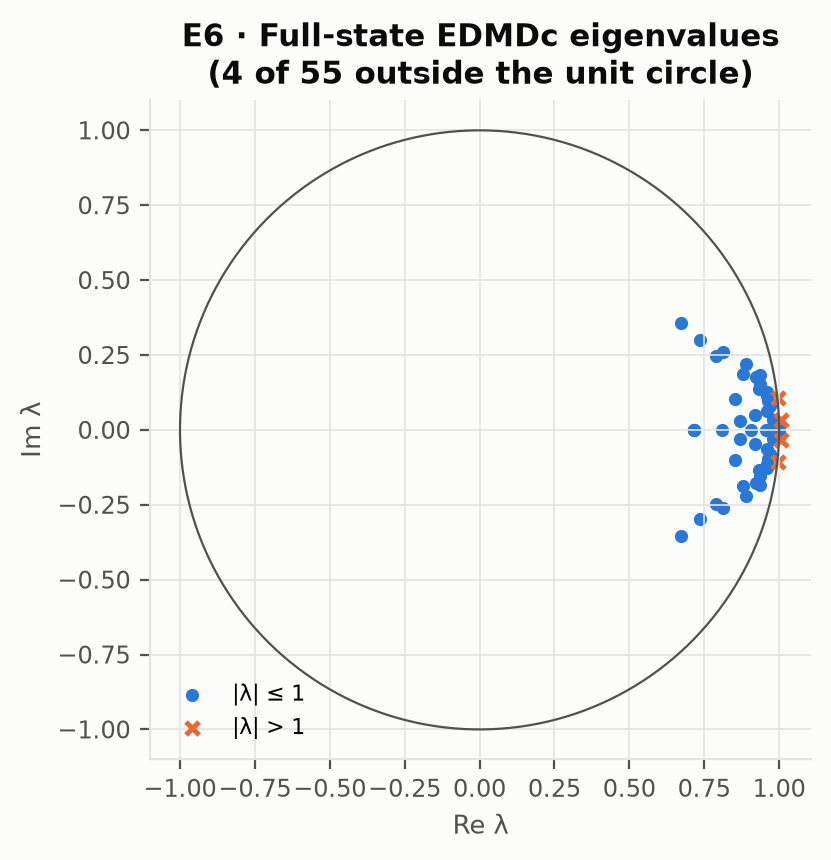
\includegraphics[width=0.45\linewidth]{figures/e6_full_edmdc_eigs.png}
\caption{Eigenvalues of the learned full-state EDMDc matrix. Crosses lie outside the unit circle, so their modes grow.}\label{fig:eigs}
\end{figure}

\paragraph{H4 (less data): supported, with one exception.} Figure~\ref{fig:eff} repeats the training with 2, 5, 10, 20 and 40 episodes and measures the error at a 0.5\,s horizon. The residual model trained on only 10 episodes (error 0.42) is already better than the full-state model trained on all 40 (0.48). This matters because data from failed flights is scarce: such flights often end in a crash. The same advantage of residual models has been reported for soft robots, ground vehicles and quadrupeds~\cite{bruder2025residual,fu2025residual,narayanan2026rkmpc}; we confirm it in the spinning regime. The curves are not monotone: at 5 episodes the full-state model is slightly better (0.93 against 1.02).

\begin{figure}[h]
\centering
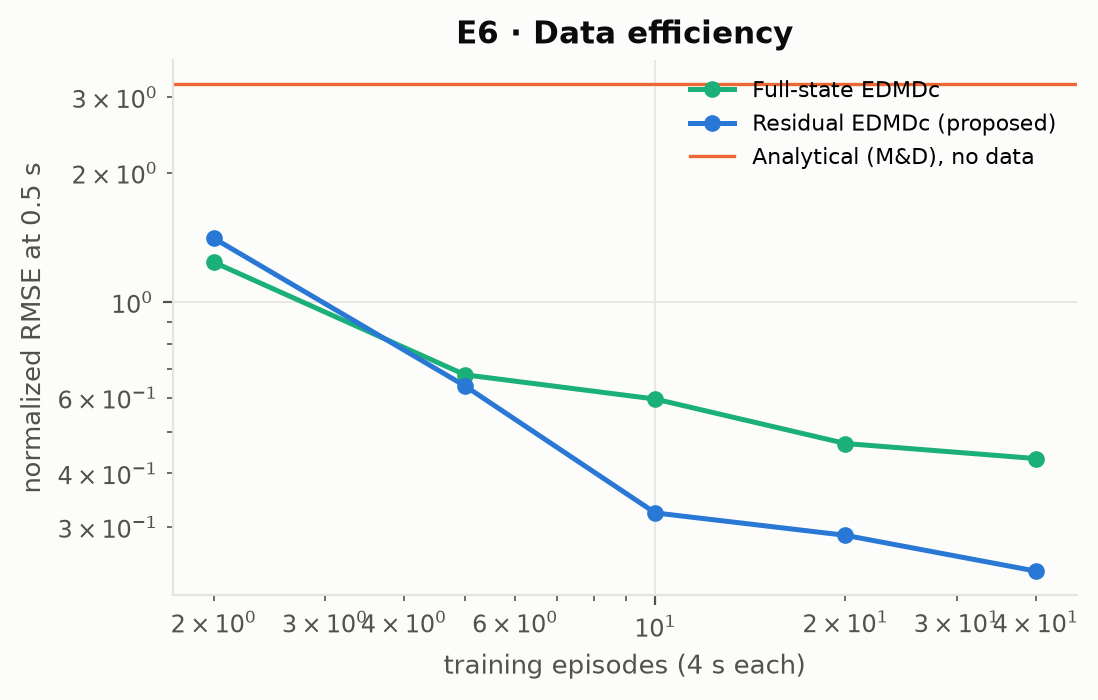
\includegraphics[width=0.55\linewidth]{figures/e6_data_efficiency.png}
\caption{Prediction error at 0.5\,s against the number of training episodes (family A). The flat line is the physics model, which uses no data.}\label{fig:eff}
\end{figure}

\paragraph{Generalization: not achieved.} On the held-out plant B, both models trained on plant A are \emph{worse} than the physics model (Table~\ref{tab:pred}, right). The learned correction is specific to the plant it saw: it ``corrects'' B as if it were A, which makes things worse. Training on randomized plants, one random plant per episode, does not solve this. It helps the residual model on B only up to about 100\,ms (error 3.68 against 4.31 for the physics model) and makes both learned models worse on A (the full-state model trained this way even diverges, spectral radius 1.028). The likely reason is that a single state sample does not reveal which plant the drone is: the motor time constant and the thrust loss show only in how the state changes over several steps. A static regression then learns an average correction that fits no plant well. This points to online adaptation: because the residual is linear in $W$, it can be updated during flight by recursive least squares. Online-adapted Koopman models exist for healthy quadrotors~\cite{jin2025dekc} and for loss-of-effectiveness faults~\cite{lee2024koopmanftmpc}.

\subsection{What this means for RQ1}
\begin{plain}
On the drone it was trained on, learning only the error of the physics model gives the best predictions from 0.1 to 1\,s, and with 10 training episodes it is more accurate than learning everything from 40 episodes. But the learned correction does not carry over to a drone with different parameters. In its current form it is a calibration for one vehicle, not a general model of rotor failure.
\end{plain}
